 \section{A szimulátor bemutatása} 
 A prototípus algoritmus fejlesztése MATLAB környezetben történt, ami később
 referenciaként szolgál.
 Alap MATLAB utasításokat használva több órát vesz igénybe a szimuláció
 futtatása.
 A MATLAB Parallel Toolbox-nak segítségével a szimulációt lehetséges
 párhuzamosan több processzormagon futtatni. Ezzel párszoros sebesség
 növekezés érhető el.
 A következőkben magát az algoritmust és az OpenCL keretrendszerben történő
 implementációját mutatjuk be.
 Majd az eredmények bemutatása során kerül összevetésre kerül a MATLAB
 referencia, a MATLAB Parallel Toolbox segítséggel, az OpenCL processzoron és
 az OpenCL GPU-n való futtatási ideje.
	
	\subsection{A lépések részletezése} 
		\subsubsection{Interpoláció}
		A korábban elmondottak alapján a felületet további mérési pontokkal egészítjük ki.
		Az extra mérési pontokat a legegyszerűbb síklapos közelítéssel alkothatjuk meg,
		a magasságmérési felbontás figyelembevételével.
		A szimulátorban egy általánosabb módszert alkalmazunk,
		ami egy 2D-s mozgó átlagoló szűrővel való simítás.
		A szűrővel aluláteresztést tudunk elérni, ami a minta magasságának
		mintavételezése utáni rekonstrukcióját jelenti. Egy ilyen interpoláció
		eredményét láthatjuk a \ref{fig:33pont}. ábrán. 
		
		\begin{figure}[!ht]
			\centering
			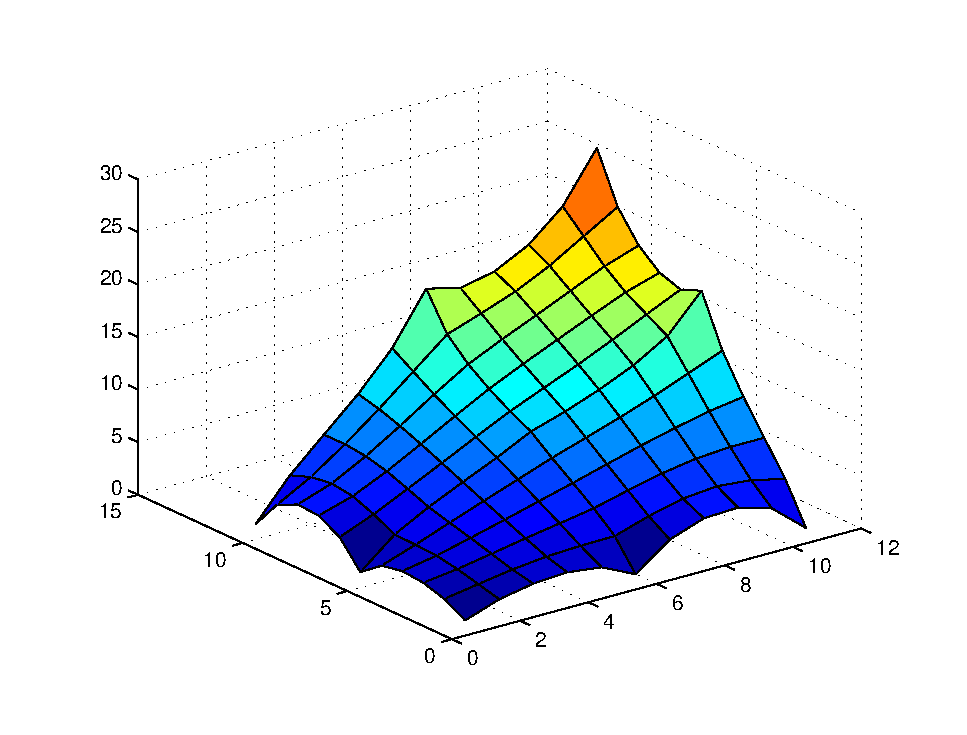
\includegraphics[width=0.95\columnwidth]{kepek/3x3_interpol.eps}
			\caption{$3\times3$ mérési pont $11\times11$ pontba való interpolációja}
			\label{fig:33pont}
		\end{figure}
		
		\subsubsection{A szimulálandó tér mérete}
		A szimulálandó tér (hasáb) magasságát a következő két mennyiség közül a
		nagyobbikkal határoztuk meg:
		\begin{itemize}
			\item Középső pont fölött lévő tű közepének magassága,
			\item A ($3\times3$) környezet legalacsonyabb és legmagasabb pontjának
			különbsége.
		\end{itemize}
		
		\begin{figure}[!h]
			\centering
			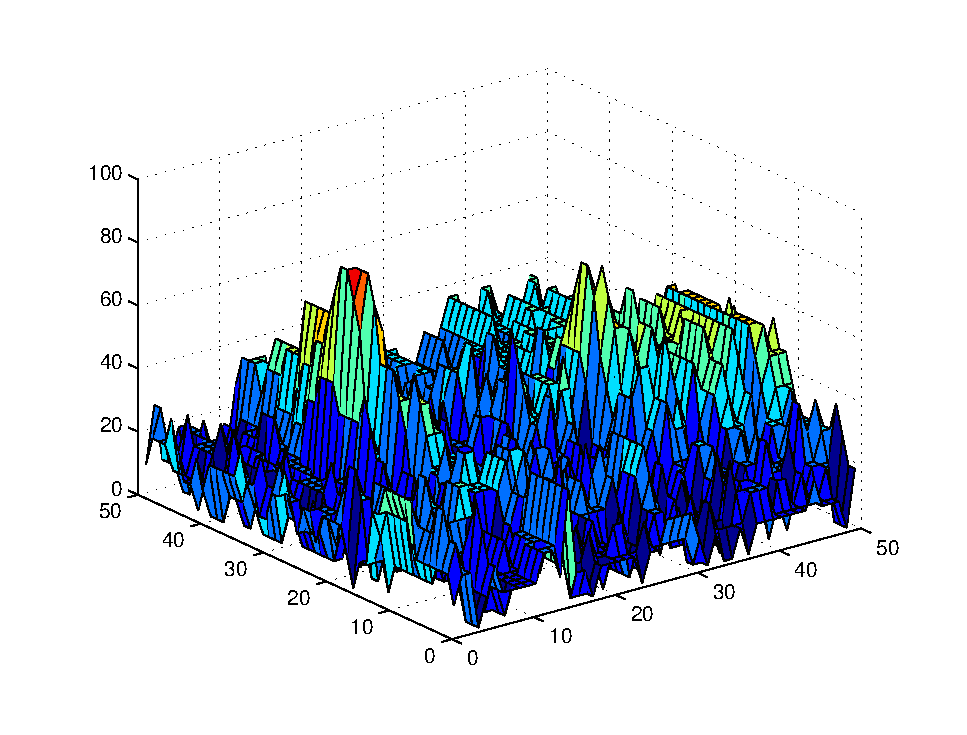
\includegraphics[width=0.45\columnwidth]{kepek/dimage.eps}
			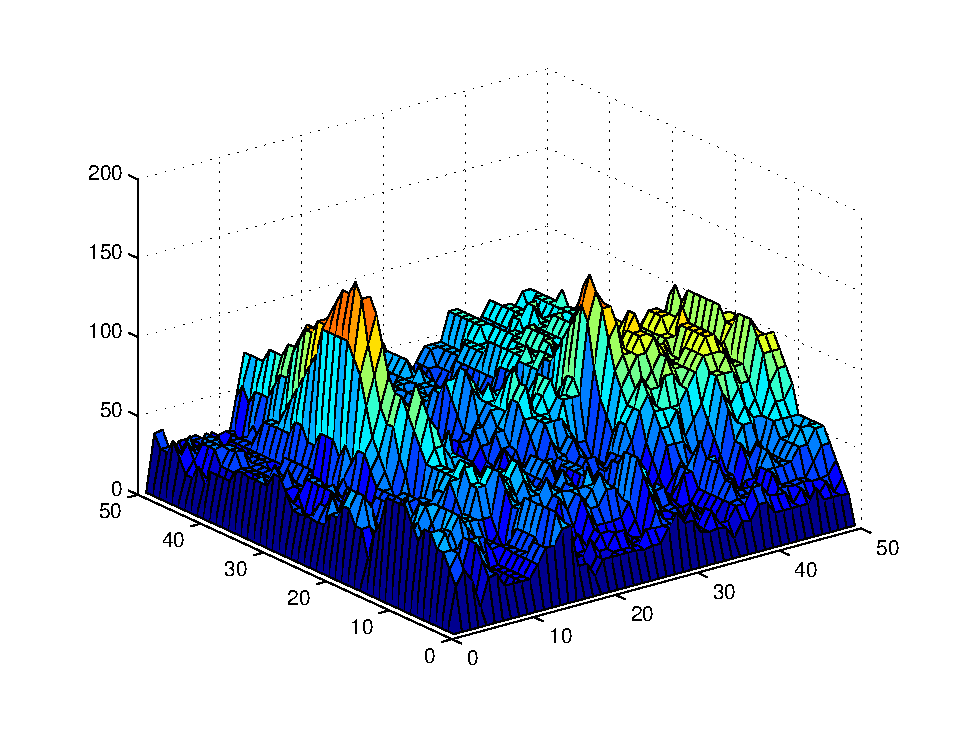
\includegraphics[width=0.45\columnwidth]{kepek/numh.eps}
			\caption{A magasságmérés eredményének részlete (balra) és a hozzá tartozó
			szimulálandó tér magassága.}
		\end{figure}
		
		\subsubsection{Iteratív megoldó algoritmus}
		Az iterációhoz a térháló pontjaihoz két mátrixot (tömbböt) rendelünk, ami a
		pontok potenciáljának aktuális ($\mathbf{U_{now}}$) és előző ($\mathbf{U_{prev}}$)
		értékeit tartalmazza.
		Az aktuális értékeket \eqref{eq:2} szerint számítjuk, majd az egész térre
		számítjuk az előzővel vett különbségének négyzetösszegét (normáját). E mérték
		képviseli a konvergencia szintjét, amit az iteráció során vizsgálva jutunk el a
		kívánt konvergencia szintre.
		Ha nem értük el a konvergencia szintet, akkor az előző két mátrixot
		felcserélve iterálunk tovább.
		
		\subsubsection{Adatok mentése}
		Tesztelhetőségi megfontolások végett a nem csak a tűre ható erőt (villamos
		térerősséget) exportáljuk, hanem a konvergencia szintjének változását és az
		interpolált felületet is. Az exportálandó menyiségek könnyen kézben tartható
		mérete miatt egyszerű CSV fájlként kerülnek mentésre. Ezen fájlok további
		poszt-processzálása MATLAB avagy munkalap kezelő szoftverrel is elvégezhető.
		
	
	\subsection{OpenCL architektúrája}
		Az Open Computing Language (OpenCL) keretrendszer \cite{opencl} közös
		nyelvet, magas szintű programozási interfészt és hardware absztrakciót nyújt a fejlesztőknek
		adat- vagy feladat párhuzamos számítások gyorsítására különböző
		számítóegységen (CPU, GPU, FPGA, DSP, \ldots).
		Az OpenCL modellje a különböző ``device''-okat, amik több ``compute unit''-ot
		(processzor-magot) tartalmaznak heterogén módon kezeli. 
		
		\begin{figure}[!ht]
			\centering
			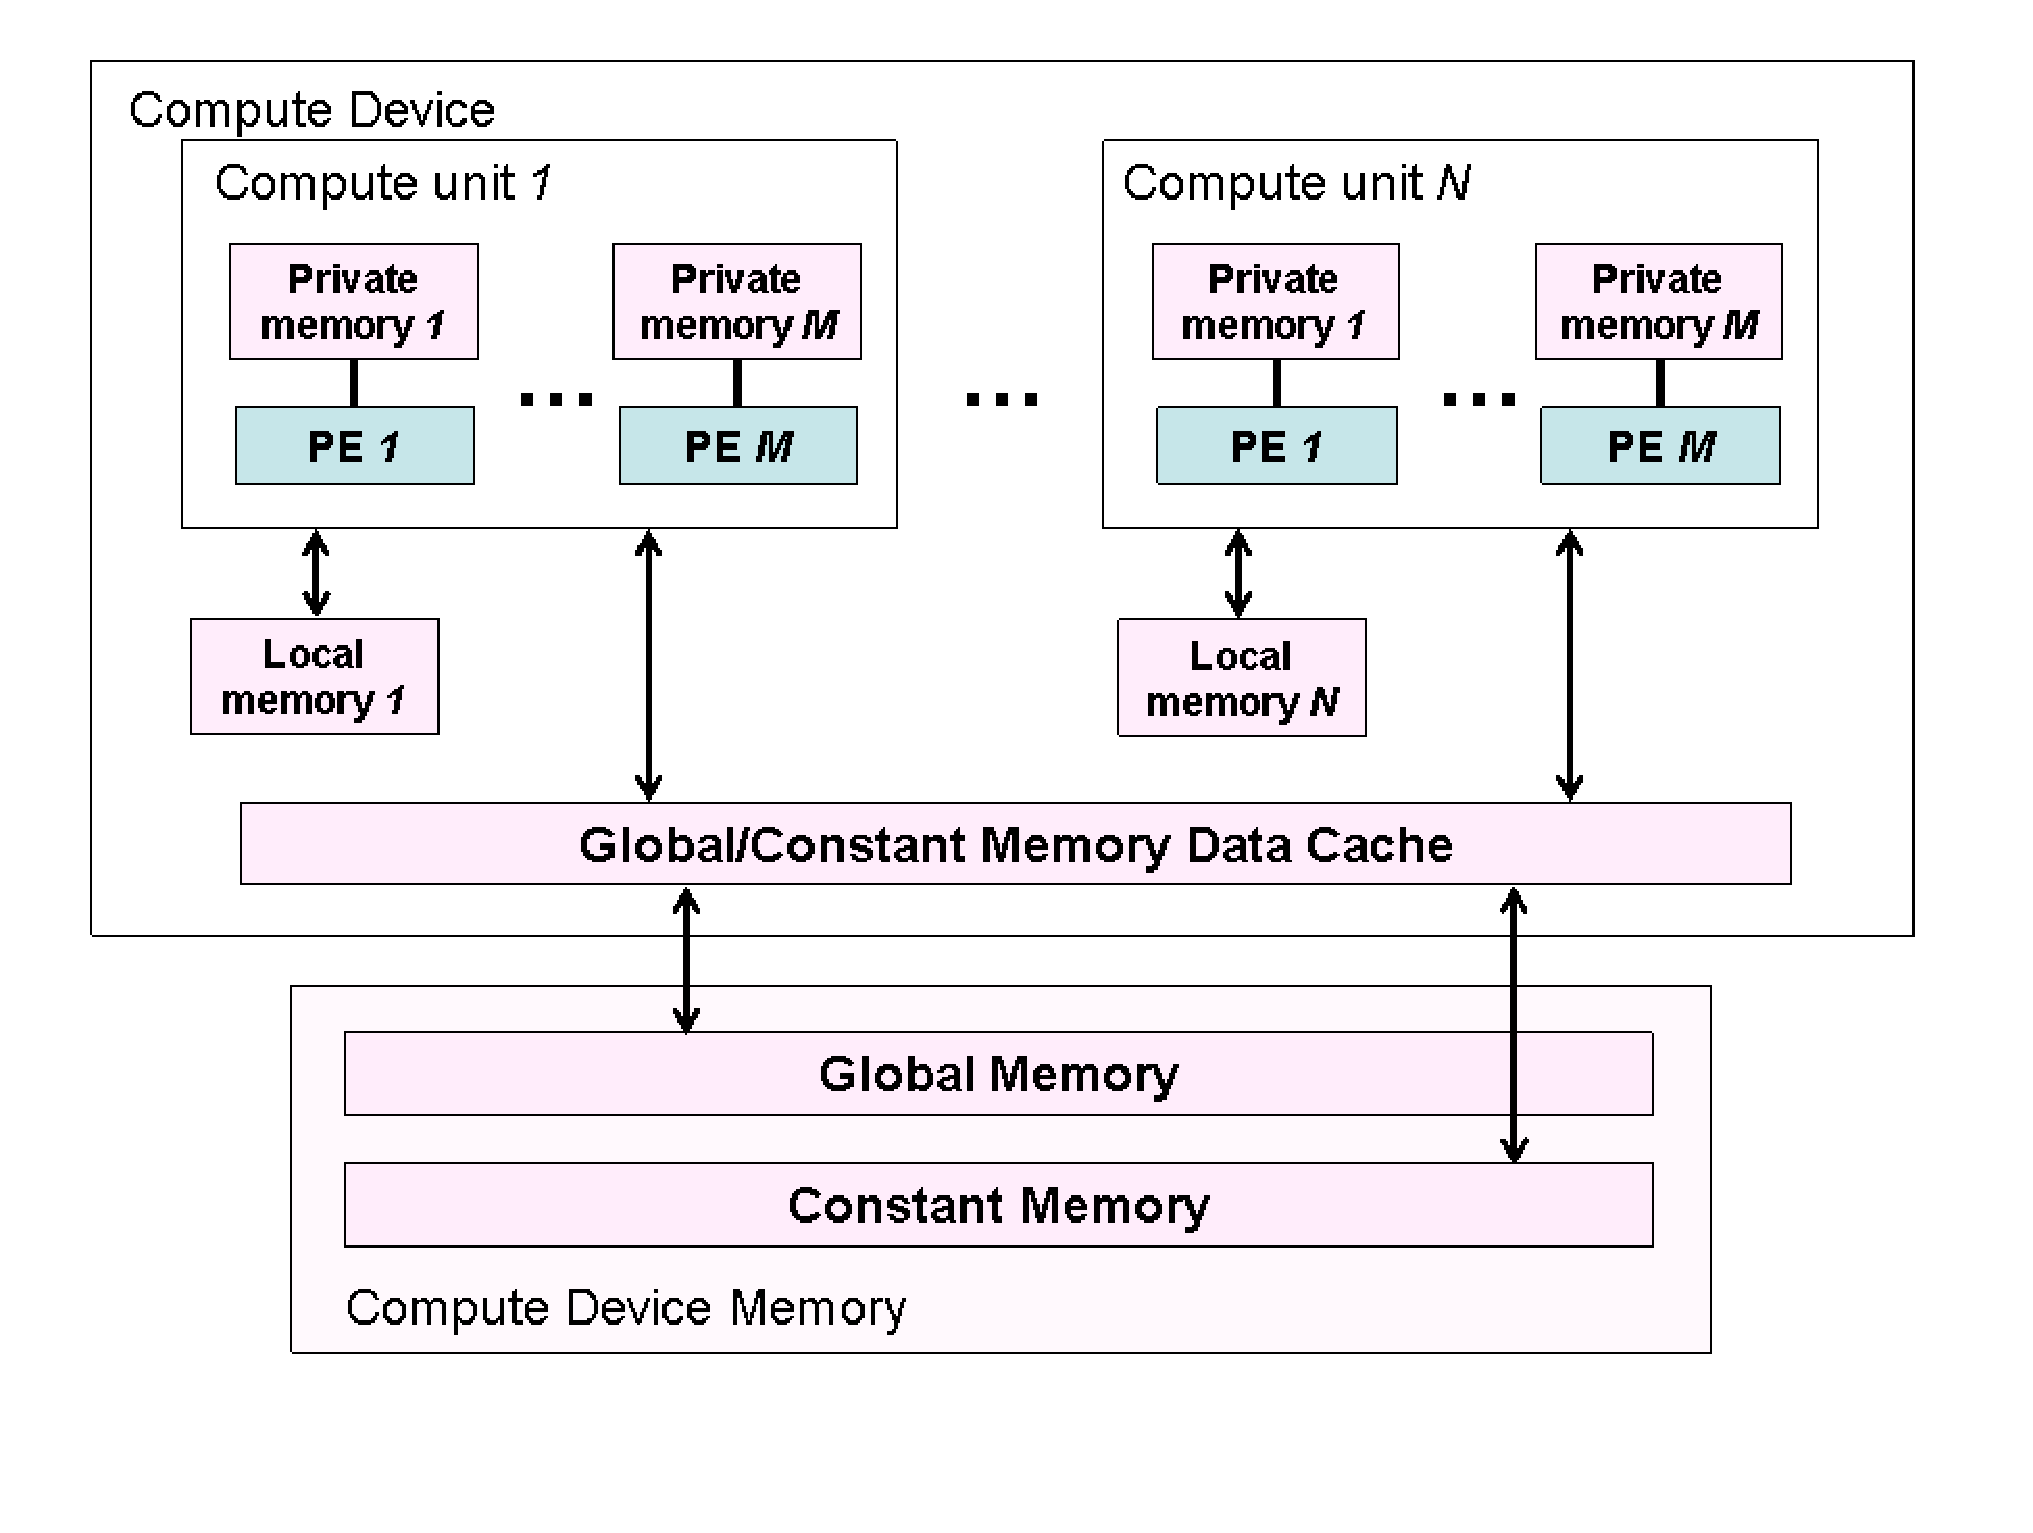
\includegraphics[width=0.95\columnwidth]{kepek/opencl_device.eps}
			\caption{OpenCL ``device'' architektúra \cite{Web:khronos}} 
			\label{fig:device} 
		\end{figure}
		
		A ``compute unit''-ok kiéheztetésének elkerülés végett (több ezer)
		``work-item'' virtuális osztozik rajta.
		Továbbá ezen ``work-item''-ek ``work-group''-okba vannak rendezve, később
		részletezett megfontolások végett.
		A ``compute unit'' kiéhesztetését a ``device''-on található memória chipek lassúsága okozza.
		Ennek hárdveres megoldása a több szintű prediktív cache memória beiktatása a
		``compute unit'' és a külső memória közé.
		Mivel a bank szervezett külső memóriák hozzáférési ideje relatíve nagy
		így a memória szervezésére nagy hangsúlyt kell fektetni.
		
		Az OpenCL négy memória szintet különböztet meg, ami az
		\ref{table:mem} táblázatban és az \ref{fig:device}. ábrán látható.
		Ahhoz, hogy a rendszerben rejlő teljesítményt kihozzuk három fontos kérdést
		kell a szimulátor magjának implementálásakor megválaszolnunk:
		\begin{itemize}
			\item \textbf{Mennyit?}: Tisztában kell lennünk az aktuális
			memória fogyasztással és a szükséges memóriamérettel.
			\item \textbf{Honnan-hova?}: Fontos, hogy a lehető legközelebb legyen az adat
			a ``work-item''-hez.
			\item \textbf{Mikor?}: Mivel a memória művelet alatt a ``work-item'' nem
			dolgozik, így átadja a helyét egy másiknak. Ennek a megfelelő
			szinkronizációjával nagyobb kihasználtság érhető el (load balance).
		\end{itemize}
		
		\begin{table}[!t]
		\renewcommand{\arraystretch}{1.3}
		% if using array.sty, it might be a good idea to tweak the value of
		% \extrarowheight as needed to properly center the text within the cells
		\caption{OpenCL memória szintek}
		\label{table:mem}
		\centering
		% Some packages, such as MDW tools, offer better commands for making tables
		% than the plain LaTeX2e tabular which is used here.
		\resizebox{\columnwidth}{!}{
		\begin{tabular}{l|l|l|l|l}
				 & Global & Constant & Local & Private\\ \hline
			Host & Dinamikusan R/W & Din. R/W & Din. R/W & \\
			Kernel & R/W & Statikusan R & Satik. R/W & Statik. R/W\\
			Sebesség & Lassú & Gyors & Gyors & Regiszter\\
			Méret & $1$ Gbyte $<$ & $\sim64$ Kbyte& $\sim16$ Kbyte & $<1$ Kbyte
		\end{tabular}
		}
		\end{table}
		

		
		OpenCL keretrendszerben történő programozás során két programot kell írnunk.
		Az egyik a ``host''-on fut, ami elvégzi a probléma összeállítását, memória
		allokálását, argumentumok beállítását és a másik program a kernel meghívását a
		``device''-on.
		A kernel futása végeztével a ``host'' program kiolvassa a ``device''-ból
		a kívánt eredményt.
		
	\subsection{Implementációhoz szükséges megfontolások}
		
		A következőkben egy kissebb teljesítményű notebook videókártyát veszek
		alapul a megfontolások demonstrálására. Ez az nVidia GeForce 330M, 
		575 MHz-en futó 48 CUDA core-al, 1024GB memóriával és
		OpenCL 1.0 kompatibilitással.
		A videókártya továbbiakban fontos paraméterei a \ref{table:vcard}. táblázatban
		látható.
		
		\begin{table}[!t]
		\renewcommand{\arraystretch}{1.3}
		% if using array.sty, it might be a good idea to tweak the value of
		% \extrarowheight as needed to properly center the text within the cells
		\caption{nVidia GeForce 330M OpenCL tulajdonságai}
		\label{table:vcard}
		\centering
		% Some packages, such as MDW tools, offer better commands for making tables
		% than the plain LaTeX2e tabular which is used here.
		\begin{tabular}{l|r}
			MAX\_COMPUTE\_UNITS & 6\\
			MAX\_WORK\_GROUP\_SIZES & 512 512 64\\
			GLOBAL\_MEM\_SIZE & 1073020928\\
			MAX\_CONSTANT\_BUFFER\_SIZE & 65536\\
			LOCAL\_MEM\_SIZE & 16384
		\end{tabular}
		\end{table}
		
		
		
		Ha a tér ahol a laplace egyenletet meg kell oldanunk nagyon nagy, akkor
		érdemes szétbontani kissebb alterekre és azokhoz rendelni egy-egy
		``work-item''-eket. Mivel a diszkrét laplace egyenlet egy pontja a szomszédos
		pontokkal szoros kapcsolatban van, így az összefüggő ``work-item"-eket egy
		``work-group''-ba érdemes szervezni, mivel így az átlapolódó pontok értékét a
		szomszédos ``work-item'' is tudják írni és olvasni. Az ilyen típusú
		problémának méretét a MAX\_WORK\_GROUP\_SIZES tulajdonság korlátozza.
		
		Jelen esetben a mérési eredmény egy pontjához tartozó tér átlagosan
		$11\times11\times30$ pontból áll.
		Tehát a korábbi nem áll fenn és egyszerű megfeleltetéssel szétoszthatjuk a
		feladatot.
		A teljes tér $512\times512\times11\times11\times30$ méretű, ami $951k$ pont.
		A tárolásához single-precision mellett ennek a számnak a 4-szerese
		szükségeltetik byte-okban mérva. Mivel ez a videókártyán nem áll
		rendelkezésre, így szétbontjuk kissebb feladatrészekre.
		
		Ezen feladatrészek méretét egy paraméter állításával lehet változtati és az
		implementált algoritmus ettől generikusan függ.
		Emellett az interpoláció mértéke is generikusan paraméterrel állítható.
		Az algoritmus generikusságát csupán a futási időben történő dinamikus memória
		allokációval lehetséges megvalósítani. A korábban említettek végett (\ref{table:mem} táblázat)
		az allokáció csak a ``host'' programban történhet.
	
	\subsection{Memória szervezés}
		\subsubsection{Csak globális memória használata}
		Az algoritmus pszeudó kódjának direkt leképezése esetén a ``host''-on
		allokálunk memóriát a ``device'' globális memóriájában.
		Majd a megfelelő adatokat ide másoljuk és a kernel is itt ír és olvas.
		A problémát a globális memória nagy hozzáférési ideje jelenti, ami miatt sok
		``work-item'' tétlenül a memóriára fog várakozni.
		Ilyenkor az egy mérési pontra vonatkoztatott szimulációs idő a
		referenciánál is lassabb.
		\subsubsection{Globális memória és adott esetben lokális memória használata}
		Kis erőfeszítéssel nagy javulást lehet elérni, ha a mérési ponthoz tartozó
		szimulációs tér éppen belefér a lokális memóriába.
		Tehát, mielött az \ref{eq:2} szerinti iteratív megoldót futtatnánk először a
		globális memóriából a lokális memóriába töltjük át a kérdéses pontokat, majd
		számolunk rajt és a végén visszatöltjük a globális memóriába.
		E javítással a referenciával azonos sebességet tudunk elérni.
		\subsubsection{Globális memória és minden adódó alkalomkor a lokális memória használata}
		Nagyobb erőfeszítést igényel, hogy a globális memórival való kommunikációt a
		lokális memória közbeékelésével tegyünk minden alkalomkor.
		Ezt úgy lehet felfogni, mintha a globális memóriát lokális memória méretű
		kvantumokban tudnám csak elérni.
		Ekkor nagy odafigyelést kíván a memóriacímzés megfelelő prgramozása, de
		eredményképp gyorsulás elérhető. \\
		
		Összegezve elmondható, hogy az aktuálisan használt adat tárolását a lehető
		legközelebb kell tartani a ``compute-unit''-hoz.
	
